% This is part of Un soupçon de mathématique sans être agressif pour autant
% Copyright (c) 2012-2013
%   Laurent Claessens
% See the file fdl-1.3.txt for copying conditions.

\EpsOrPdfincludegraphics[width=\linewidth]{BO_perspective}

Note : savoir si deux droites dans l'espace sont perpendiculaires n'est pas au programme. Dans ce chapitre nous allons donc nous en tenir qu'à des choses simples.

\vspace{1cm}

% This is part of Un soupçon de mathématique sans être agressif pour autant
% Copyright (c) 2013
%   Laurent Claessens
% See the file fdl-1.3.txt for copying conditions.

\begin{wrapfigure}[3]{r}{5.0cm}
   \vspace{-0.5cm}        % à adapter.
   \centering
   \input{Fig_MEzTDZC.pstricks}
\end{wrapfigure}

À l'aide du cube ci-contre :
\begin{enumerate}
    \item
        Quelle est la nature du triangle \( AEF\) ? 
    \item
        Quelle est la nature du quadrilatère \( ABGH\) ?
    \item
        Est-ce que vous pouvez trouver trois points de ce cube formant un triangle équilatéral ?
    \item
        Si ce cube fait \unit{3}{\meter} de côté, quelle est la longueur de la «grande» diagonale \( [AG]\) ?
\end{enumerate}



%+++++++++++++++++++++++++++++++++++++++++++++++++++++++++++++++++++++++++++++++++++++++++++++++++++++++++++++++++++++++++++ 
\section{Ce qui est dans un plan}
%+++++++++++++++++++++++++++++++++++++++++++++++++++++++++++++++++++++++++++++++++++++++++++++++++++++++++++++++++++++++++++

Les trois suivantes permettent d'affirmer que tel point ou telle droite est dans un plan.
\begin{enumerate}
    \item
        Si \( d\) est une droite et \( P\) est un point d'un plan, alors la parallèle à \( d\) passant par \( P\) est encore dans le plan.
    \item
        Si \( P\) et \( Q\) sont deux points d'un plan, alors toute la droite \( (PQ)\) est encore dans ce plan.
    \item
        Deux droites non parallèles situées dans un même plan sont sécantes.
\end{enumerate}

%---------------------------------------------------------------------------------------------------------------------------
\subsection{Position relative de deux plans}
%---------------------------------------------------------------------------------------------------------------------------

\begin{definition}
    Deux plans sont \defe{parallèles}{parallèle!deux plans} soit si ils sont confondus, soit si ils n'ont aucun point commun. Si ils n'ont aucun point communs, nous disons qu'ils sont \defe{strictement parallèles}{parallèle!strictement}
\end{definition}


\begin{Aretenir}
    Deux plans non parallèles se coupent en une droite.
\end{Aretenir}

\begin{multicols}{2}

    \begin{center}
        Plans parallèles
    \end{center}
   % Des plans parallèles sont soit confondus, soit n'ont aucun point communs.
    

%Les plans \( (AEB)\) et \( (DHC)\) ci-contre sont parallèles.

\columnbreak

%The result is on figure \ref{LabelFigPositionPlansTvKvah}. % From file PositionPlansTvKvah
%\newcommand{\CaptionFigPositionPlansTvKvah}{<+Type your caption here+>}
    \begin{center}
\input{Fig_PositionPlansTvKvah.pstricks}
    \end{center}


\end{multicols}

\begin{multicols}{2}
    \begin{center}
        Plans sécants
    \end{center}
 %   L'intersection de deux plans sécants (non confondus) est une droite.

  %  L'intersection des plans \( (ABG)\) et \( (DCG)\) ci-contre est la droite \( (HG)\).

    \columnbreak

%The result is on figure \ref{LabelFigPositionPlansqSltxa}. % From file PositionPlansqSltxa
%\newcommand{\CaptionFigPositionPlansqSltxa}{<+Type your caption here+>}
    \begin{center}
\input{Fig_PositionPlansqSltxa.pstricks}
    \end{center}

\end{multicols}

%---------------------------------------------------------------------------------------------------------------------------
\subsection{Position relative de deux droites}
%---------------------------------------------------------------------------------------------------------------------------

Deux droites peuvent être soit dans un même plan, soit ne pas être dans le même plan. Deux droites contenues dans un même plan sont dires \defe{coplanaires}{coplanaire}.

%///////////////////////////////////////////////////////////////////////////////////////////////////////////////////////////
\subsubsection{Droites coplanaires}
%///////////////////////////////////////////////////////////////////////////////////////////////////////////////////////////

Deux droites coplanaires respectent la géométrie usuelle. Elles peuvent être parallèles ou sécantes.

\begin{multicols}{2}
    \begin{center}
        Droites parallèles dans le plan \( (EBC)\)
    \end{center}

    \columnbreak

    \begin{center}
        \input{Fig_IDqyzXM.pstricks}
    \end{center}
\end{multicols}

\begin{multicols}{2}
    \begin{center}
        Droites sécantes dans le plan \( (AEH)\)
    \end{center}

    \columnbreak

    \begin{center}
        \input{Fig_ETfnbsh.pstricks}
    \end{center}
\end{multicols}

\begin{Aretenir}
    À propos de droites coplanaires :
    \begin{enumerate}
        \item
            Deux droites sécantes sont toujours coplanaires.
        \item
            Deux droites parallèles sont coplanaires.
    \end{enumerate}
\end{Aretenir}

\begin{proof}

    \begin{enumerate}
        \item

    Soient \( d\) et \( d'\) deux droites sécantes dans l'espace. Soit \( K\) leur point d'intersection; soit \( A\), un autre point sur \( d\) et \( B\) un autre point sur \( d'\).

    Le plan défini par les points \( A\), \( K\) et \( B\) contient les deux droites.

    \item

        Si \( d\) et \( d'\) sont parallèles nous considérons les points \( P\) et \( Q\) sur \( d\) et un point \( A\) sur \( d'\). D'une part droite \( d\) est dans le plan \( (PQA)\) parce que deux de ses points y sont. D'autre part la droite parallèle à \( d\) passant par \( A\) est la droite \( d'\) et est dans le plan comprenant la droite \( d\) et le point \( A\), c'est à dire le plan \( (PQA)\) également.

    \end{enumerate}
\end{proof}

%///////////////////////////////////////////////////////////////////////////////////////////////////////////////////////////
    \subsubsection{Droites non coplanaires}
%///////////////////////////////////////////////////////////////////////////////////////////////////////////////////////////
    
Deux droites non coplanaires ne peuvent pas être sécantes, ni parallèles.

\begin{multicols}{2}
    \begin{center}
        Il est possible pour deux droites dans l'espace d'être ni sécantes ni parallèles.
    \end{center}

    \columnbreak

    \begin{center}
        \input{Fig_ENQhxmG.pstricks}
    \end{center}
\end{multicols}

%---------------------------------------------------------------------------------------------------------------------------
\subsection{Position relative d'une droite et un plan}
%---------------------------------------------------------------------------------------------------------------------------

\begin{definition}
    Une droite est \defe{parallèle}{parallèle!droite et plan} à un plan lorsque soit la droite est contenue dans le plan, soit elle n'a aucun point commun avec le plan.
\end{definition}

\begin{multicols}{2}

    \begin{center}
        Droite et plan sécants
    \end{center}

    La droite \( (FD)\) intersecte le plan \( (ABH)\) au point \( M\).
%he result is on figure \ref{LabelFigfigureBCtCTZo}. % From file figureBCtCTZo
%\newcommand{\CaptionFigfigureBCtCTZo}{<+Type your caption here+>}

    \columnbreak
    \begin{center}
\input{Fig_figureBCtCTZo.pstricks}
    \end{center}
\end{multicols}

\begin{multicols}{2}

    \begin{center}
        Droite et plan parallèles
    \end{center}

    La droite \( (HC)\) et le plan \( (EBF)\) sont parallèles.

    \columnbreak
    \begin{center}
%The result is on figure \ref{LabelFigfigureASkECWS}. % From file figureASkECWS
%\newcommand{\CaptionFigfigureASkECWS}{<+Type your caption here+>}
\input{Fig_figureASkECWS.pstricks}
    \end{center}
\end{multicols}

\begin{multicols}{2}

    \begin{center}
        Droite contenue dans un plan
    \end{center}

    La droite \( (EB)\) est contenue dans le plan \( (AEF)\).

    \columnbreak
    \begin{center}
%The result is on figure \ref{LabelFigfigureCSIQETx}. % From file figureCSIQETx
%\newcommand{\CaptionFigfigureCSIQETx}{<+Type your caption here+>}
\input{Fig_figureCSIQETx.pstricks}
    \end{center}
\end{multicols}

\begin{definition}
    Une droite est \defe{perpendiculaire}{perpendiculaire!droite et plan} à un plan si elle est perpendiculaire à deux droites non confondues du plan.
\end{definition}

\begin{Aretenir}
    Si la droite \( d\) est perpendiculaire au plan \( \Omega\), alors toutes les droites du plan \( \Omega\) sécantes avec \( d\) sont perpendiculaires à \( d\).
\end{Aretenir}

\begin{remark}
    Seules deux droites peuvent être ni parallèle ni sécantes.
\end{remark}

%+++++++++++++++++++++++++++++++++++++++++++++++++++++++++++++++++++++++++++++++++++++++++++++++++++++++++++++++++++++++++++ 
\section{Surfaces dans un cube}
%+++++++++++++++++++++++++++++++++++++++++++++++++++++++++++++++++++++++++++++++++++++++++++++++++++++++++++++++++++++++++++

La figure \ref{LabelFigDesSections} montre un cube. Êtes-vous capables de donner la nature des surfaces coloriées ?
\newcommand{\CaptionFigDesSections}{Exercice de vision dans l'espace.}
\input{Fig_DesSections.pstricks}
Le triangle vert est isocèle et rectangle parce que deux de ses côtés sont des arrêtes du cube. Le triangle rouge est plus troublant, mais il est équilatéral : ses trois côtés sont des diagonales des faces du cube. Notez que \emph{sur le dessin}, les trois côtés ont des longueur différentes.

%+++++++++++++++++++++++++++++++++++++++++++++++++++++++++++++++++++++++++++++++++++++++++++++++++++++++++++++++++++++++++++
\section{Les règles de la perspective cavalière}
%+++++++++++++++++++++++++++++++++++++++++++++++++++++++++++++++++++++++++++++++++++++++++++++++++++++++++++++++++++++++++++

Lorsque nous dessinons en trois dimension, nous prenons les conventions suivantes qui définissent la \defe{\wikipedia{fr}{Perspective_cavalière}{perspective cavalière}}{perspective!cavalière}.

\begin{Aretenir}
    D'abord nous choisissons
    \begin{enumerate}
        \item
            Nous choisissons un \defe{angle de fuite}{angle!de fuite} \( \alpha\) qui sera entre \unit{30}{\degree} et \( \unit{45}{\degree}\) avec l'horizontale\footnote{Sur une feuille à carreaux, le plus simple est de prendre \unit{45}{\degree}.}.
        \item
            Un \defe{coefficient de réduction}{coefficient de réduction} que nous noterons \( k\) et qui sera compris entre \( 0\) et \( 1\).
    \end{enumerate}

    Ensuite nous prenons les correspondances suivantes entre la réalité et le dessin :
    \begin{center}
        \begin{tabular}{|p{7.5cm}|p{7.5cm}|}
            \hline
            {\bf dans la réalité}&{\bf sur le dessin}\\
            \hline\hline
            Segment caché  & Segment pointillé\\
            \hline
            Segment parallèle à la feuille de dessin & Segment représenté en vraie grandeur\\
            \hline
            Segment perpendiculaire à la feuille de dessin & Segment faisant un angle \( \alpha\) avec l'horizontale.\\
            \hline
            Une arrête de longueur \( l\) perpendiculaire à la feuille de dessin & Une arrête de longueur \( k\times l\) faisant un angle \( \alpha\) avec l'horizontale.\\
            \hline
        \end{tabular}
    \end{center}
\end{Aretenir}

\begin{minipage}{0.485\textwidth}
    Un carré fait un demi-centimètre. 
    \begin{itemize}
        \item Quel est l'angle de fuite utilisé ?
        \item Quel est le coefficient de réduction utilisé ?
    \end{itemize}
\end{minipage}
\hspace{1mm}
\begin{minipage}{0.6\textwidth}
    \center
    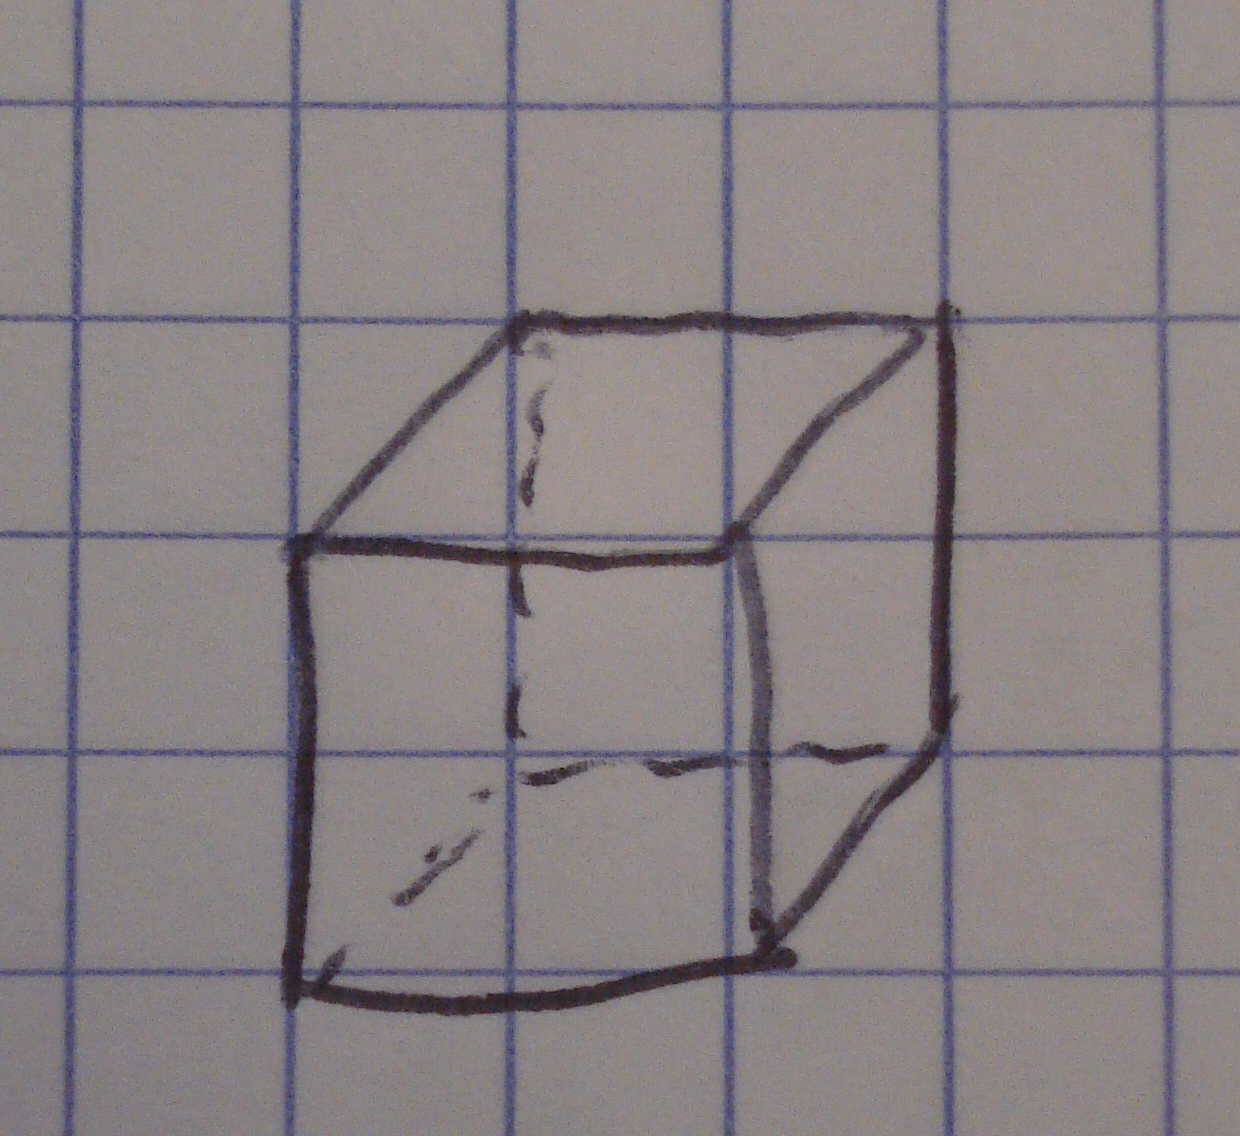
\includegraphics[width=0.6\textwidth]{cube_quadrill.png}
\end{minipage}

\begin{propriete}
    La perspective cavalière respecte les conditions suivantes.
    \begin{enumerate}
        \item
             Deux segments parallèles dans la réalité sont représentés par deux segments parallèles sur le dessin.
         \item
             Trois points alignés dans la réalité sont représentés par trois points alignés sur le dessin.
         \item
             Si \( M\) est le milieu du segment \( [AB]\) dans la réalité, alors \( M\) est le milieu du segment \( [AB]\) dans la réalité.
         \item
             La perspective cavalière respecte les proportions. C'est à dire que si le segment \( [AB]\) est \( p\) fois plus grand que le segment \( [CD]\) dans la réalité, alors il sera \( p\) fois plus grand sur le dessin.
    \end{enumerate}
\end{propriete}

Le cube de la figure \ref{LabelFigCubeLFZuiW} est dessiné avec \( \alpha=\unit{45}{\degree}\) et \( k=0.5\). Notez que les côtés parallèles restent parallèles.
\newcommand{\CaptionFigCubeLFZuiW}{Les segments perpendiculaires à la feuille sont de longueur moitié des autres.}
\input{Fig_CubeLFZuiW.pstricks}

La perspective cavalière n'est pas parfaite; il est aisé de créer des illusions d'optique comme celle de la figure \ref{LabelFigIllusionNHwEtp}. % From file IllusionNHwEtp
\newcommand{\CaptionFigIllusionNHwEtp}{Une petite illusion d'optique facile.}
\input{Fig_IllusionNHwEtp.pstricks}
